\documentclass[tikz, border=7pt]{standalone}
\usepackage{tikz}

\begin{document}
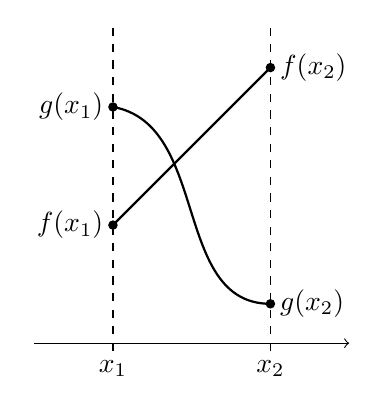
\begin{tikzpicture}

% talnalína
\draw [->] (0,1) -- (4,1);
\draw [dashed] (1,0.9) -- (1,5);
\node [below] at (1,0.9) {$x_1$};
\draw [dashed] (3,0.9) -- (3,5);
\node [below] at (3,0.9) {$x_2$};
% punktar
\draw [fill] (1,4) circle [radius=1.5pt] node [left] {$g(x_1)$};
\draw [fill] (1,2.5) circle [radius=1.5pt] node [left] {$f(x_1)$};
\draw [fill] (3,1.5) circle [radius=1.5pt] node [right] {$g(x_2)$};
\draw [fill] (3,4.5) circle [radius=1.5pt] node [right] {$f(x_2)$};
% föll
\draw [thick] (1,4) to [out=350, in=180] (3,1.5);
\draw [thick] (1,2.5) to [out=45, in=225] (3,4.5);

\end{tikzpicture}
\end{document}
